\documentclass[answers,12pt,a4paper]{exam}
\usepackage[T1]{fontenc}
\usepackage{longtable}
\usepackage{graphicx}
\usepackage{geometry}
\usepackage{multicol}
\usepackage{relsize}
\usepackage{pgf}
\usepackage{fancyvrb}
\usepackage{verbatim}

\usepackage{hyperref}
%\urlstyle{same}  % don't use monospace font for urls
\setlength{\parindent}{0pt}
\setlength{\parskip}{6pt plus 2pt minus 1pt}

\geometry{margin=2.54cm}

\fvset{tabsize=2}
%\fvset{fontsize=\relsize{-2}}
\fvset{frame=single}

\title{Exercises on Design Patterns - Part I}
\author{Week 05}
\date{2018}
\newcommand{\code}{/Users/keith/Documents/Courses/sdp/repo/worksheets/dp-one/kotlin/src}
\newcommand{\codesol}{/Users/keith/Documents/Courses/sdp/repo/worksheets/dp-one-sol/src}

%http://hp.fciencias.unam.mx/~alg/bd/patrones.pdf
\begin{document}
\maketitle

In these exercises we will be examining the following design patterns:
\begin{itemize}
\item Adapter,
\item Decorator,
\item Factory Method,
\item Observer, and
\item Singleton.
\end{itemize}
The source code snippets listed below are written using the Kotlin language; similar 
versions in Scala can be found on the source code repository under the \verb!worksheets/dp-one! folder. 

\section*{Short form questions}

\begin{questions}
\question % 2.1 - Combine with next question
Write down three differences between \emph{abstract classes} and \emph{interfaces/traits} in Kotlin/Scala.
Provide examples to illustrate your answer.

\begin{solution}
An abstract class with no non-abstract methods is similar to an interface in terms of its 
utility. However, note the following.
\begin{itemize}
\item
A class can implement any number of interfaces but can subclass at most one abstract class.
\item
An abstract class can have non-abstract methods, which are usually instances of the 
\textsc{TEMPLATE METHOD} pattern (more of which later). 
All the methods of an interface are abstract, whether or not this declaration is explicit.
\item
An abstract class can declare instance variables that its subclasses inherit. 
An interface cannot declare instance variables, although it can establish 
\verb!static final! fields.
\item
An abstract class can define constructors; an interface cannot.
\item
An abstract class's visibility can be \verb!public!, \verb!protected!, \verb!private!, 
or none (package); an interface's visibility must be \verb!public! or none (package).
\item
An abstract class can have methods whose visibility is \verb!protected!, 
\verb!private!, or none (package); every method in an interface must be \verb!public!.
\item
An abstract class inherits from \verb!Object!, including such methods as \verb!clone()! 
and \verb!equals()!.
\end{itemize}
\end{solution}

\question % 2.2 e, f, g
Are the following \emph{true} or \emph{false}? 

\begin{parts}
\part Every interface must have at least one method.

\begin{solution}
\emph{False}. An interface with no methods is a \emph{marker interface}. 
Sometimes, a method high in a class hierarchy, such as \verb!Object.clone()!, 
is not appropriate for every subclass. You can create a marker interface that 
requires subclasses to opt in or to opt out of participation in such a method. 
The \verb!clone()! method on \verb!Object! requires subclasses to opt in, 
declaring that they implement the \verb!Cloneable! marker interface.	
\end{solution}

\part An interface can declare instance fields that an implementing class must also
declare.

\begin{solution}
\emph{False}. 
An interface cannot declare instance fields, although it can create constants 
by declaring fields that are \verb!static! and \verb!final!.	
\end{solution}

\part Although you can't instantiate an interface, an interface definition can
declare constructor methods that require an implementing class to provide 
constructors with given signatures.	

\begin{solution}
\emph{False}. 
It might be a good idea, but there is no way for an interface to require 
implementing classes to provide any particular constructors.
\end{solution}
\end{parts}
Provide examples to illustrate your answers.

\question % 2.3 - reword to make clearer what is required. Combine with next question.
Provide an example of an interface with methods that do not imply responsibility 
on the part of the implementing class to take action on behalf of the caller or 
to return a value.

\begin{solution}
An interface does not define a contract between the caller and the implementing 
class when the interface is used to \emph{register} for notification. In this case, 
the implementing class may need to take an action in response to a method call, 
but it is generally not performing a service for the caller.

For example, a class that implements the \verb!MouseMotionListener! interface from
\verb!java.awt.event! must implement the methods: 
\begin{Verbatim}
	public void mouseDragged(MouseEvent e)
	public void mouseMoved(MouseEvent e)
\end{Verbatim}	
The presence of these methods does not imply that the methods will take an 
action when a client calls them. In fact, it would not be uncommon to react to the 
\verb!mouseDragged()! method but to ignore to calls to the 
\verb!mouseMoved()! method.	
\end{solution}

\question % 2.4
What is the value of a stub class like \verb!WindowAdapter! which is composed of methods that do nothing?

%\VerbatimInput[label="stub/WindowListener.java"]{\code/stub/WindowListener.kt}
%
%\VerbatimInput[label="stub/WindowAdapter.java"]{\code/stub/WindowAdapter.kt}

\begin{solution}
A class that implements \verb!WindowListener! must implement all the methods the 
interface declares, even if the class will ignore these methods when called. 
The \verb!WindowAdapter! class ignores all the methods in \verb!WindowListener!. 
This lets a subclass implement only the methods that it wants to react to. 
The anonymous class in the code below can react to only the \verb!windowClosing()! 
event, without having to implement dummy methods for the other methods specified in the 
\verb!WindowListener! interface.
\begin{Verbatim}
public static void listen(Frame f) {
    f.addWindowListener(
             new WindowAdapter() {
                public void windowClosing(WindowEvent e){
					System.exit(0);
				} 
			}
	);
}
\end{Verbatim}
This code registers with the frame an instance of an anonymous \verb!WindowAdapter! 
subclass that overrides the \verb!windowClosing()! method. 
The value of the \verb!WindowAdapter! class is that it makes it easy to create 
a subclass that reacts to only the relevant window events.	
\end{solution}

\question % 8.1
How can you prevent other developers from constructing new instances of your class? 
Provide appropriate examples to illustrate your answer.

\begin{solution}
To prevent other developers from instantiating your class, 
create a single constructor with private visibility. Note that if you create other, 
non-private constructors or create no constructors at all, other developers will likely 
be able to re-instantiate your class.
\end{solution}

%\question 
%Using the \verb!java.util.Observable} and \verb!java.util.Observer} 
%classes/interfaces show how one object can be informed of updates to another object.
%
%\begin{solution}
%Standard example from the Java Tutorial.	
%\end{solution}
%
%\question 
%``The \emph{Observer} pattern supports the \emph{MVC} pattern''. State if this statement
%is \emph{true} or \emph{false} and support your answer by use of an appropriate example.
%
%\begin{solution}
%\emph{True}. Any example which shows that the View-Controller provides an observer with 
%the Model the observable. This can also work the other way around with the Controller being the
%class \emph{watched}.
%\end{solution}
%
\question % 16.1
Provide examples of two commonly used Kotlin/Scala methods that return a new object.

\begin{solution}
Many answers are possible, but \verb!toString()! is probably the most commonly used method 
that creates a new object. For example, the following code creates a new \verb!String! object:
\begin{Verbatim}
	String s = new Date().toString();
\end{Verbatim}
The creation of strings often happens behind the scenes. Consider:
\begin{Verbatim}
	System.out.print(new Date());
\end{Verbatim}	
This method creates a \verb!String! object from the \verb!Date! object, 
ultimately by calling the \verb!toString()! method of class \verb!Date!. 
It is interesting to walk through this in a debugger, to see the details of what happens 
within a common \verb!print()! method.

Another method that creates a new object is \verb!clone()!. 
You may discover other methods that are ``factories'' 
for creating objects without necessarily exacting the \textsc{FACTORY METHOD} pattern.	
\end{solution}

\question 
What are the signs that a \emph{Factory Method} is at work?

\begin{solution}
\begin{itemize}
\item Creates a new object
\item Returns a type that is an abstract class or an interface
\item Is implemented by several classes	
\end{itemize}	
\end{solution}

\question % 27.1
If you want to direct output to the standard output instead of to a file, 
you can create a \verb!Writer} object that directs its output to \verb!System.out!:
\begin{Verbatim}
	val out: Writer = PrintWriter(System.out)
\end{Verbatim}	
Write a code example to define a \verb!Writer! object that wraps text at 15 characters, 
centres the text, sets the text to random casing, and directs the output to \verb!System.out!.
Which design pattern are you using?

\begin{solution}
One answer is:
\begin{Verbatim}
	Writer out = new PrintWriter(System.out);
	out = new WrapFilter(new BufferedWriter(out), 15);
	((WrapFilter) out).setCenter(true);
	out = new RandomCaseFilter(out);
\end{Verbatim}	
Alternatively:
\begin{Verbatim}
WrapFilter out =
    new WrapFilter(
        new BufferedWriter(
            new RandomCaseFilter(
                new PrintWriter(System.out))),15);
out.setCenter(true);	
\end{Verbatim}     
\end{solution}           
\end{questions}

\section*{Long form questions}

% https://www.javacodegeeks.com/2015/09/decorator-design-pattern.html
\begin{questions}
\question
The \textsc{Factory Method} pattern gives us a way to encapsulate the instantiations of 
concrete types; it encapsulates the functionality required to select and instantiate 
an appropriate class, inside a designated method referred to as a \emph{factory method}. 
The factory method selects an appropriate class from a class hierarchy based on the 
application context and other contributing factors and it then instantiates the selected class 
and returns it as an instance of the parent class type.
The advantage of this approach is that the application objects can make use of the 
factory method to gain access to the appropriate class instance. 
This eliminates the need for an application object to deal explicitly with the 
varying class selection criteria.

You are required to implement the following classes:
\begin{description}
\item[\texttt{Product}]
defines the interface of objects the factory method creates.
\item[\texttt{ConcreteProduct}]
implements the \verb!Product! interface.
\item[\texttt{Creator}]
declares the factory method, which returns an object of type \verb!Product!. 
\verb!Creator! may also define a default implementation of the factory method 
that returns a default \verb!ConcreteProduct! object.
We may call the factory method to create a \verb!Product! object.
\item[\texttt{ConcreteCreator}]
overrides the factory method to return an instance of a \verb!ConcreteProduct!.
\end{description}
Factory methods therefore eliminate the need to bind application-specific classes into your code.
The code only deals with the \verb!Product! interface (in this case); 
therefore it can work with any user-defined \verb!ConcreteProduct! classes.

\begin{solution}
	\VerbatimInput{\codesol/factory/Product.scala}
	\VerbatimInput{\codesol/factory/ConcreteProduct.scala}
	\VerbatimInput{\codesol/factory/Creator.scala}
	\VerbatimInput{\codesol/factory/ConcreteCreator.scala}
\end{solution}

\question
In this question we examine the \textsc{Singleton} design pattern.
\begin{parts}
\part
Why might you decide to \emph{lazy-initialise} a singleton instance rather than initialise 
it in its field declaration? Provide code examples of both approaches to illustrate your answer.

\begin{solution}
You might not have enough information to instantiate every singleton at static initialisation
time. A singleton might require values that are computed later in the program's execution. 
When a \verb!Factory! singleton is born, for example, 
it might have to establish connections 
with machine drivers, to set up planners, and to initialise a simulation of itself.

	\VerbatimInput{\codesol/singletonpattern/SingletonEager.scala}
	\VerbatimInput{\codesol/singletonpattern/SingletonLazy.scala}
\end{solution}
%\part
%Imagine that we now wish to use the code in a \emph{multi-threaded environment}.
%Two threads concurrently access the class, thread \verb!t1} 
%gives the first call to the \verb!getInstance()! method, it will check if the 
%static variable that holds the reference to the singleton instance is \verb!null! 
%and then gets interrupted due to some reason. 
%Another thread \verb!t2! calls the \verb!getInstance()! method successfully passes the 
%instance check and instantiates the object. Then, thread \verb!t1! wakes and 
%it also creates the object. At this time, there would be two objects of this class which
%was supposedly a singleton.
%\begin{parts}
%\part
%How could we use the \verb!synchronized! keyword to the \verb!getInstance()! method to operate 
%correctly.
%\part
%The synchronised version comes with a price as it will decrease the 
%performance of the code --- why?
%\part
%If the call to the \verb!getInstance()! method isn't causing a substantial overhead for 
%your application, then you can forget about it.
%\part
%If you want to use synchronisation (or need to), then there is another technique known as 
%\emph{double-checked locking} which reduces the use of synchronisation. With double-checked
%locking, we first check to see if an instance is created, and if not, then we synchronise.
%
%Provide a sample implementation of this technique.
%\end{parts}
%
%\begin{solution}
%	\VerbatimInput{\code/singletonpattern/SingletonLazyMultithreaded.kt}
%	
%	\VerbatimInput{\code/singletonpattern/SingletonLazyDoubleCheck.kt}
%\end{solution}
\part
There are many ways to break the singleton pattern. One is in a multi-threaded environment but 
others include:
\begin{itemize}
\item If the class is \verb!Serializable!.
\item If it is \verb!Cloneable!.
\item It can be broken by reflection.
\item If the class is loaded by multiple \emph{class loaders}.	
\end{itemize}
Try and write a class \verb!SingletonProtected! that addresses some (all?) of these issues.

\begin{solution}
\VerbatimInput{\codesol/singletonpattern/SingletonProtected.scala}	
\end{solution}
\end{parts}

\question
We now consider the \textsc{Adapter} design pattern.

A software developer, Max, has worked on an e-commerce website. 
The website allows users to shop and pay online. The site is integrated with a third party 
payment gateway, through which users can pay their bills using their credit card. 
Everything was going well, until his manager called him for a change in the project.

The manager has told him that they are planning to change the payment gateway vendor, 
and Max has to implement that in the code. The problem that arises here is that the site 
is attached to the \verb!Xpay! payment gateway which takes an \verb!Xpay! type of object. 
The new vendor, \verb!PayD!, only allows the \verb!PayD! type of objects to allow the process. 
Max doesn't want to change the whole set of a hundred classes which have reference to an 
object of type \verb!XPay!. He cannot change the third party tool provided by the payment gateway. 
The problem arises due to the incompatible interfaces between the two different parts of 
the code. To get the process to work, Max needs to find a way to make the code 
compatible with the vendor's provided API.
\medskip

\centerline{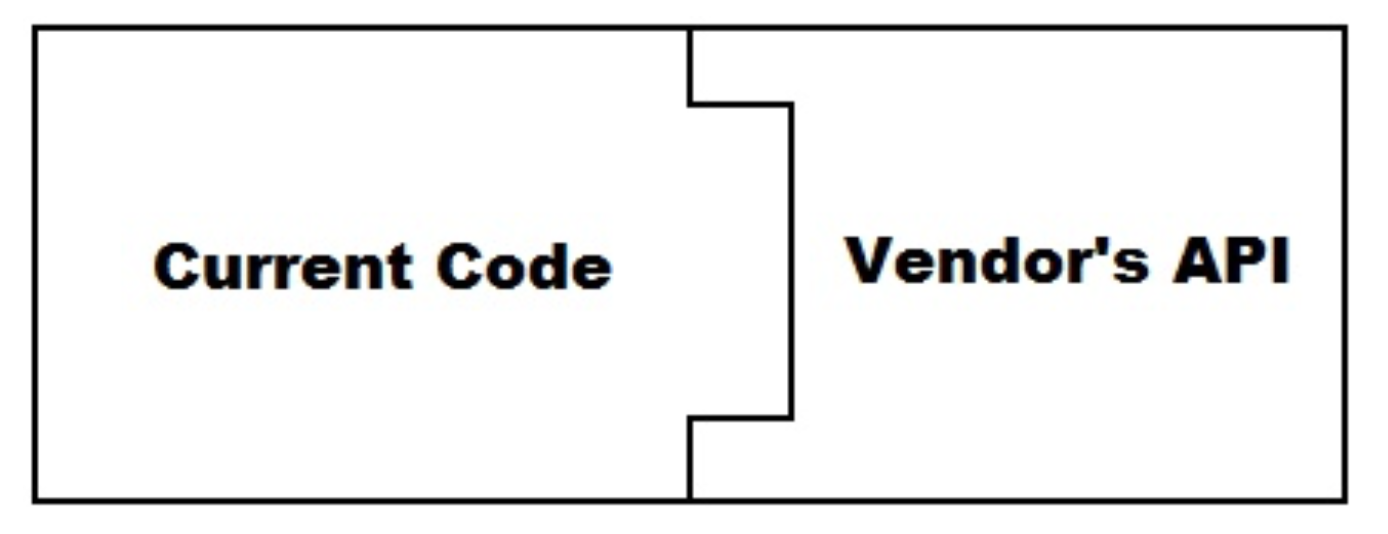
\includegraphics[width=0.4\textwidth]{images/code}}

The current code interface is not compatible with the new vendor's interface. What Max 
needs here is an \textsc{Adapter} which can sit in between the code and the vendor's API, 
enabling the transaction to proceed.

\VerbatimInput{\code/xpay/Xpay.kt}

The \verb!Xpay! interface contains setter and getter methods to get the information about 
the credit card and customer name. The interface is implemented in the following code which is 
used to instantiate an object of this type, and exposes the object to the vendor's API.

\VerbatimInput{\code/xpay/XpayImpl.kt}

New vendor's interface looks like this:

\VerbatimInput{\code/xpay/PayD.kt}

As you can see, this interface has a set of different methods which need to be implemented 
in the code. However, \verb!Xpay! objects are created by most parts of the code, 
and it is difficult (and risky) to change the entire set of classes.
We need some way, that's able to fulfil the vendor's requirement to process the payment 
and also make less or no change to the current code base. 

Your are required to use the Adapter pattern to implement a 
\verb!XpayToPayDAdapter! class to meet the requirements.
\medskip

\centerline{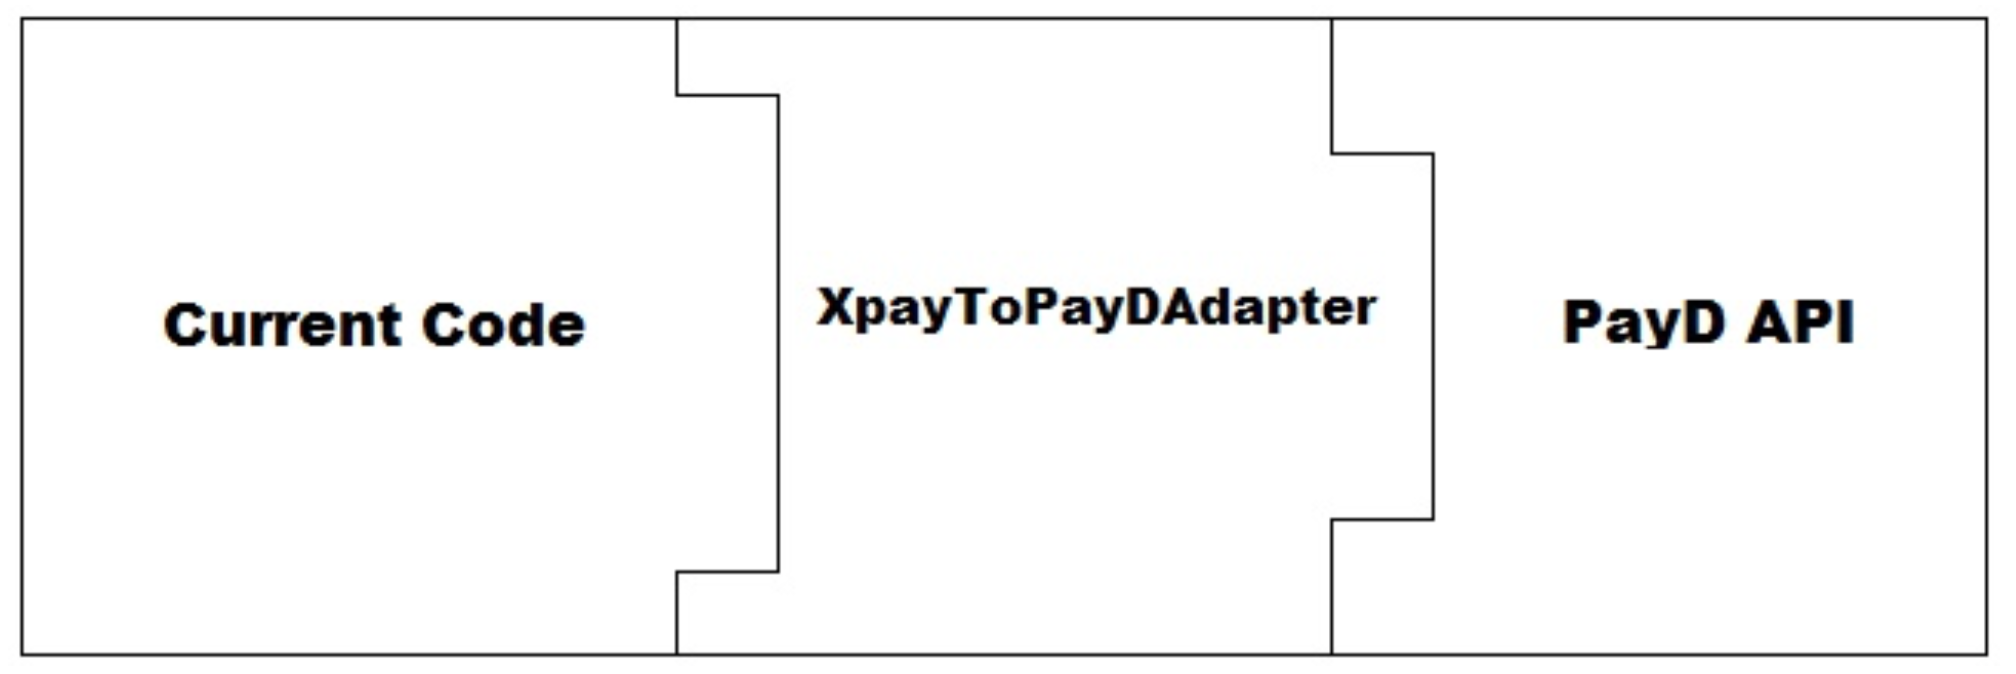
\includegraphics[width=0.5\textwidth]{images/adapt}}

\begin{solution}
\VerbatimInput{\codesol/adapterpattern/site/XpayToPayDAdapter.scala}
\end{solution}

\question
This question examines the \textsc{Observer} design pattern.

\emph{Sports Lobby} is a sports website targeted at sport lovers. 
They cover almost all kinds of sports and provide the latest news, 
information, matches scheduled dates, information about a particular player or a team. 
Now, they are planning to provide live commentary or scores of matches as an SMS service, 
but only for their premium users. Their aim is to SMS the live score, match situation, 
and important events after short intervals. As a user, you need to 
subscribe to the package and when there is a live match you will get an SMS to the 
live commentary. The site also provides an option to unsubscribe from the package 
whenever a user wants to.
As a developer, the Sport Lobby has asked you to provide this new feature for them. 
The reporters of the Sport Lobby will sit in the commentary box in the match, and they will 
update live commentary to a commentary object. As a developer your job is to 
provide the commentary to the registered users by fetching it from the commentary 
object when it's available. When there is an update, 
the system should update the subscribed users by sending them the SMS.
This situation clearly indicates a \emph{one-to-many} mapping between the match and the users, 
as there could be many users subscribed to a single match. The \textsc{Observer} design pattern 
is best suited to this situation --- you should implement this feature for 
Sport Lobby using the \textsc{Observer} pattern. 

Remember that there are four participants in the \textsc{Observer} pattern:
\begin{description}
\item[\texttt{Subject}] which is used to register observers. 
Objects use this interface to register as observers and also to remove 
themselves from being observers.
\item[\texttt{Observer}] defines an updating interface for objects that 
should be notified of changes in a subject. 
All observers need to implement the \texttt{Observer} interface. 
This interface has a method \verb!update()!, which gets called when the \verb!Subject!'s 
state changes.
\item[\texttt{ConcreteSubject}] stores the state of interest to \verb!ConcreteObserver! objects. 
It sends a notification to its observers when its state changes. 
A concrete subject always implements the \verb!Subject! interface. 
The \verb!notifyObservers()! method is used to update all the current observers 
whenever the state changes.
\item[\texttt{ConcreateObserver}] maintains a reference to a 
\verb!ConcreteSubject! object and implements the \verb!Observer! interface. 
Each observer registers with a concrete subject to receive updates.
\end{description}

\VerbatimInput{\code/observer/Observer.kt}
\VerbatimInput{\code/observer/Subject.kt}
\VerbatimInput{\code/observer/Commentary.kt}
\VerbatimInput{\code/observer/TestObserver.kt}

\begin{solution}
\VerbatimInput{\codesol/observerpattern/CommentaryObject.scala}

\VerbatimInput{\codesol/observerpattern/CommentaryObjectObservable.scala}

\VerbatimInput{\codesol/observerpattern/SMSUsers.scala}

\VerbatimInput{\codesol/observerpattern/SMSUsersObserver.scala}
	
\VerbatimInput{\codesol/observerpattern/TestObserver.scala}	
\end{solution}

\question
This question considers the \textsc{Decorator} design pattern.

You are commissioned by a pizza company make an extra topping calculator. 
A user can ask to add extra topping to a pizza and our job is to add toppings and 
increase its price using our classes.

\emph{Please note}: the main aim of the \textsc{Decorator} design pattern is to 
attach additional responsibilities to an object dynamically. 
Decorators provide a flexible alternative to sub-classing for extending functionality.
The Decorator prevents the proliferation of subclasses leading to less complexity and confusion.

For simplicity, let's create a simple \verb!Pizza! 
interface which contains only two methods:

\VerbatimInput{\code/decorator/Pizza.kt}

The \verb!getDesc! method is used to obtain the pizza's description whereas the 
\verb!getPrice} is used to obtain the price.

Provide two implementations of the \verb!Pizza! interface:
\begin{itemize}
\item \verb!SimplyVegPizza!
\item \verb!SimplyNonVegPizza!
\end{itemize}

\begin{solution}
\VerbatimInput{\codesol/decoratorpattern/SimplyVegPizza.scala}
\VerbatimInput{\codesol/decoratorpattern/SimplyNonVegPizza.scala}
\end{solution}

The decorator wraps the object whose functionality needs to be increased, 
so it needs to implement the same interface. Provide an abstract decorator class which 
will be extended by all the concrete decorators.

Now provide several implementations of \verb!PizzaDecorator! and exercise your classes
with the given test class. 
\begin{itemize}
\item \verb!Ham: PizzaDecorator!
\item \verb!Cheese: PizzaDecorator!
\item \verb!Chicken: PizzaDecorator!
\item \verb!FetaCheese: PizzaDecorator!
\item \ldots
\end{itemize}
%\VerbatimInput{\code/decorator/TestDecoratorPattern.kt}

\VerbatimInput{\code/decorator/TestDecoratorPattern.kt}

The code should result in the following output:
{\small
\begin{Verbatim}[frame=none]
Desc: SimplyVegPizza (230), Roma Tomatoes (5.20), Green Olives (5.47), Spinach (7.92)
Price: 248.59
Desc: SimplyNonVegPizza (350), Meat (14.25), Cheese (20.72), Cheese (20.72), Ham (18.12)
Price: 423.81
\end{Verbatim}
}

\begin{solution}
\VerbatimInput{\codesol/decoratorpattern/Broccoli.scala}
\VerbatimInput{\codesol/decoratorpattern/FetaCheese.scala}
\VerbatimInput{\codesol/decoratorpattern/Meat.scala}
\VerbatimInput{\codesol/decoratorpattern/RedOnions.scala}
\VerbatimInput{\codesol/decoratorpattern/SimplyVegPizza.scala}
\VerbatimInput{\codesol/decoratorpattern/Cheese.scala}
\VerbatimInput{\codesol/decoratorpattern/GreenOlives.scala}
\VerbatimInput{\codesol/decoratorpattern/RomaTomatoes.scala}
\VerbatimInput{\codesol/decoratorpattern/Spinach.scala}
\VerbatimInput{\codesol/decoratorpattern/Chicken.scala}
\VerbatimInput{\codesol/decoratorpattern/Ham.scala}
\VerbatimInput{\codesol/decoratorpattern/PizzaDecorator.scala}
\end{solution}
\end{questions}

\end{document}